\clearpage
\begin{figure}[!htbp]
 \centering
 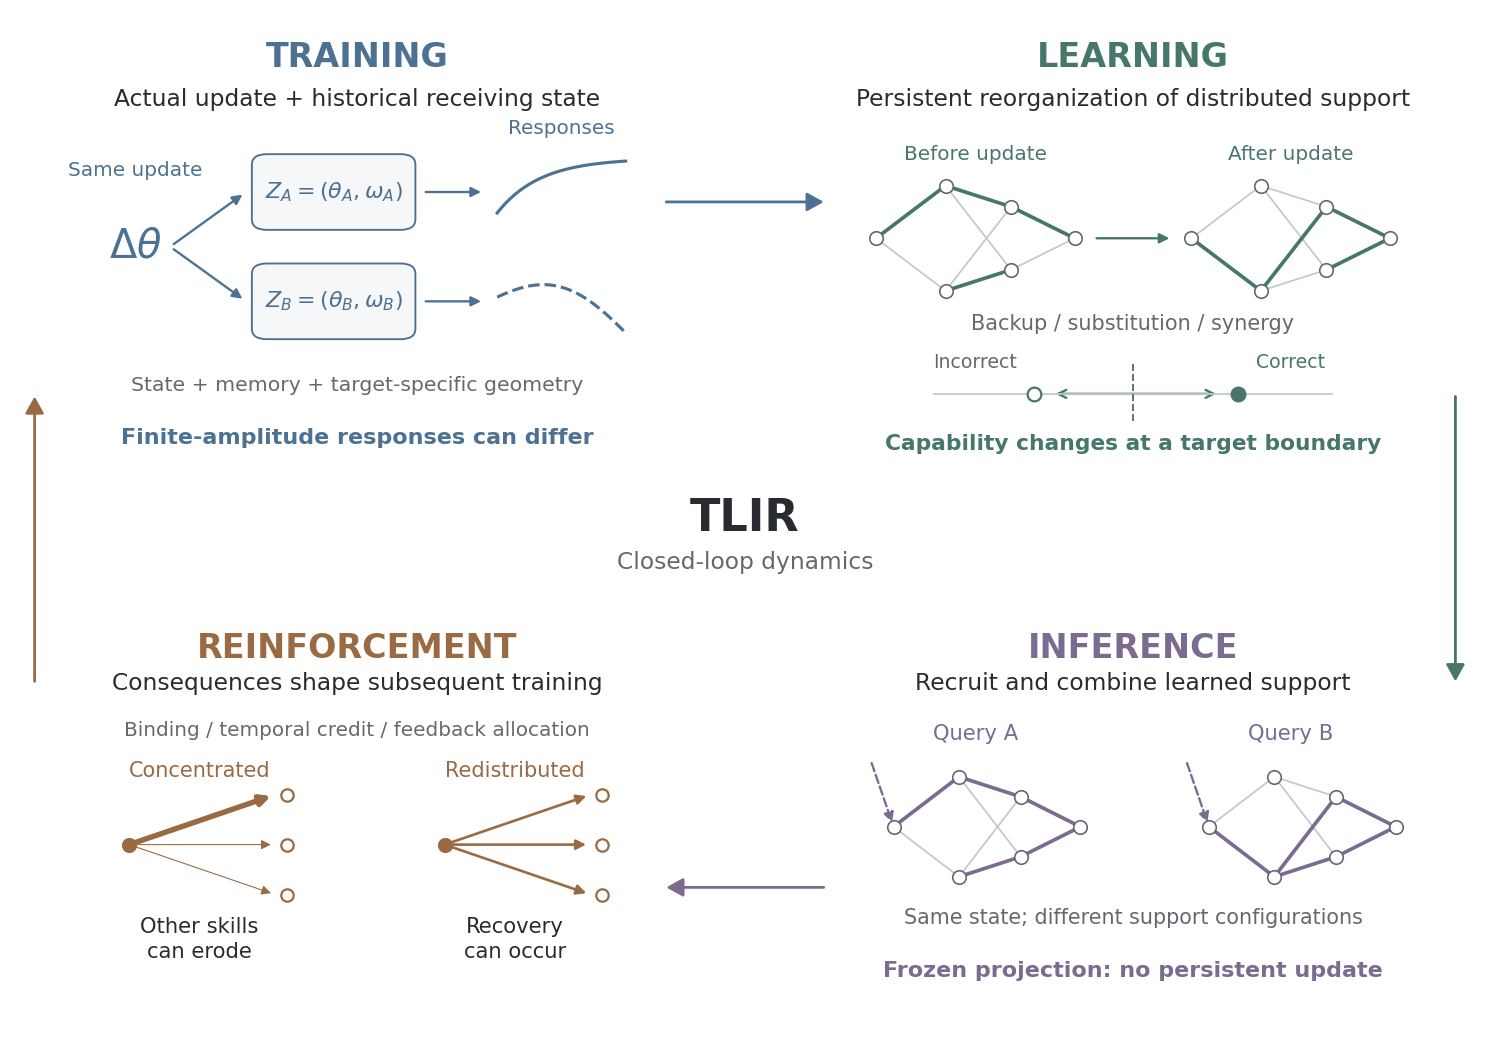
\includegraphics[width=.98\textwidth]{../figures/figure1_tlir_closed_loop.png}
 \caption{TLIR 闭环动力学。训练、学习和推理构成开环核心；强化则将模型行为产生的后果反馈至后续训练，从而形成闭环。}
 \label{fig:chain}
\end{figure}

\begin{figure}[!htbp]
 \centering
 \captionsetup{font=footnotesize}
 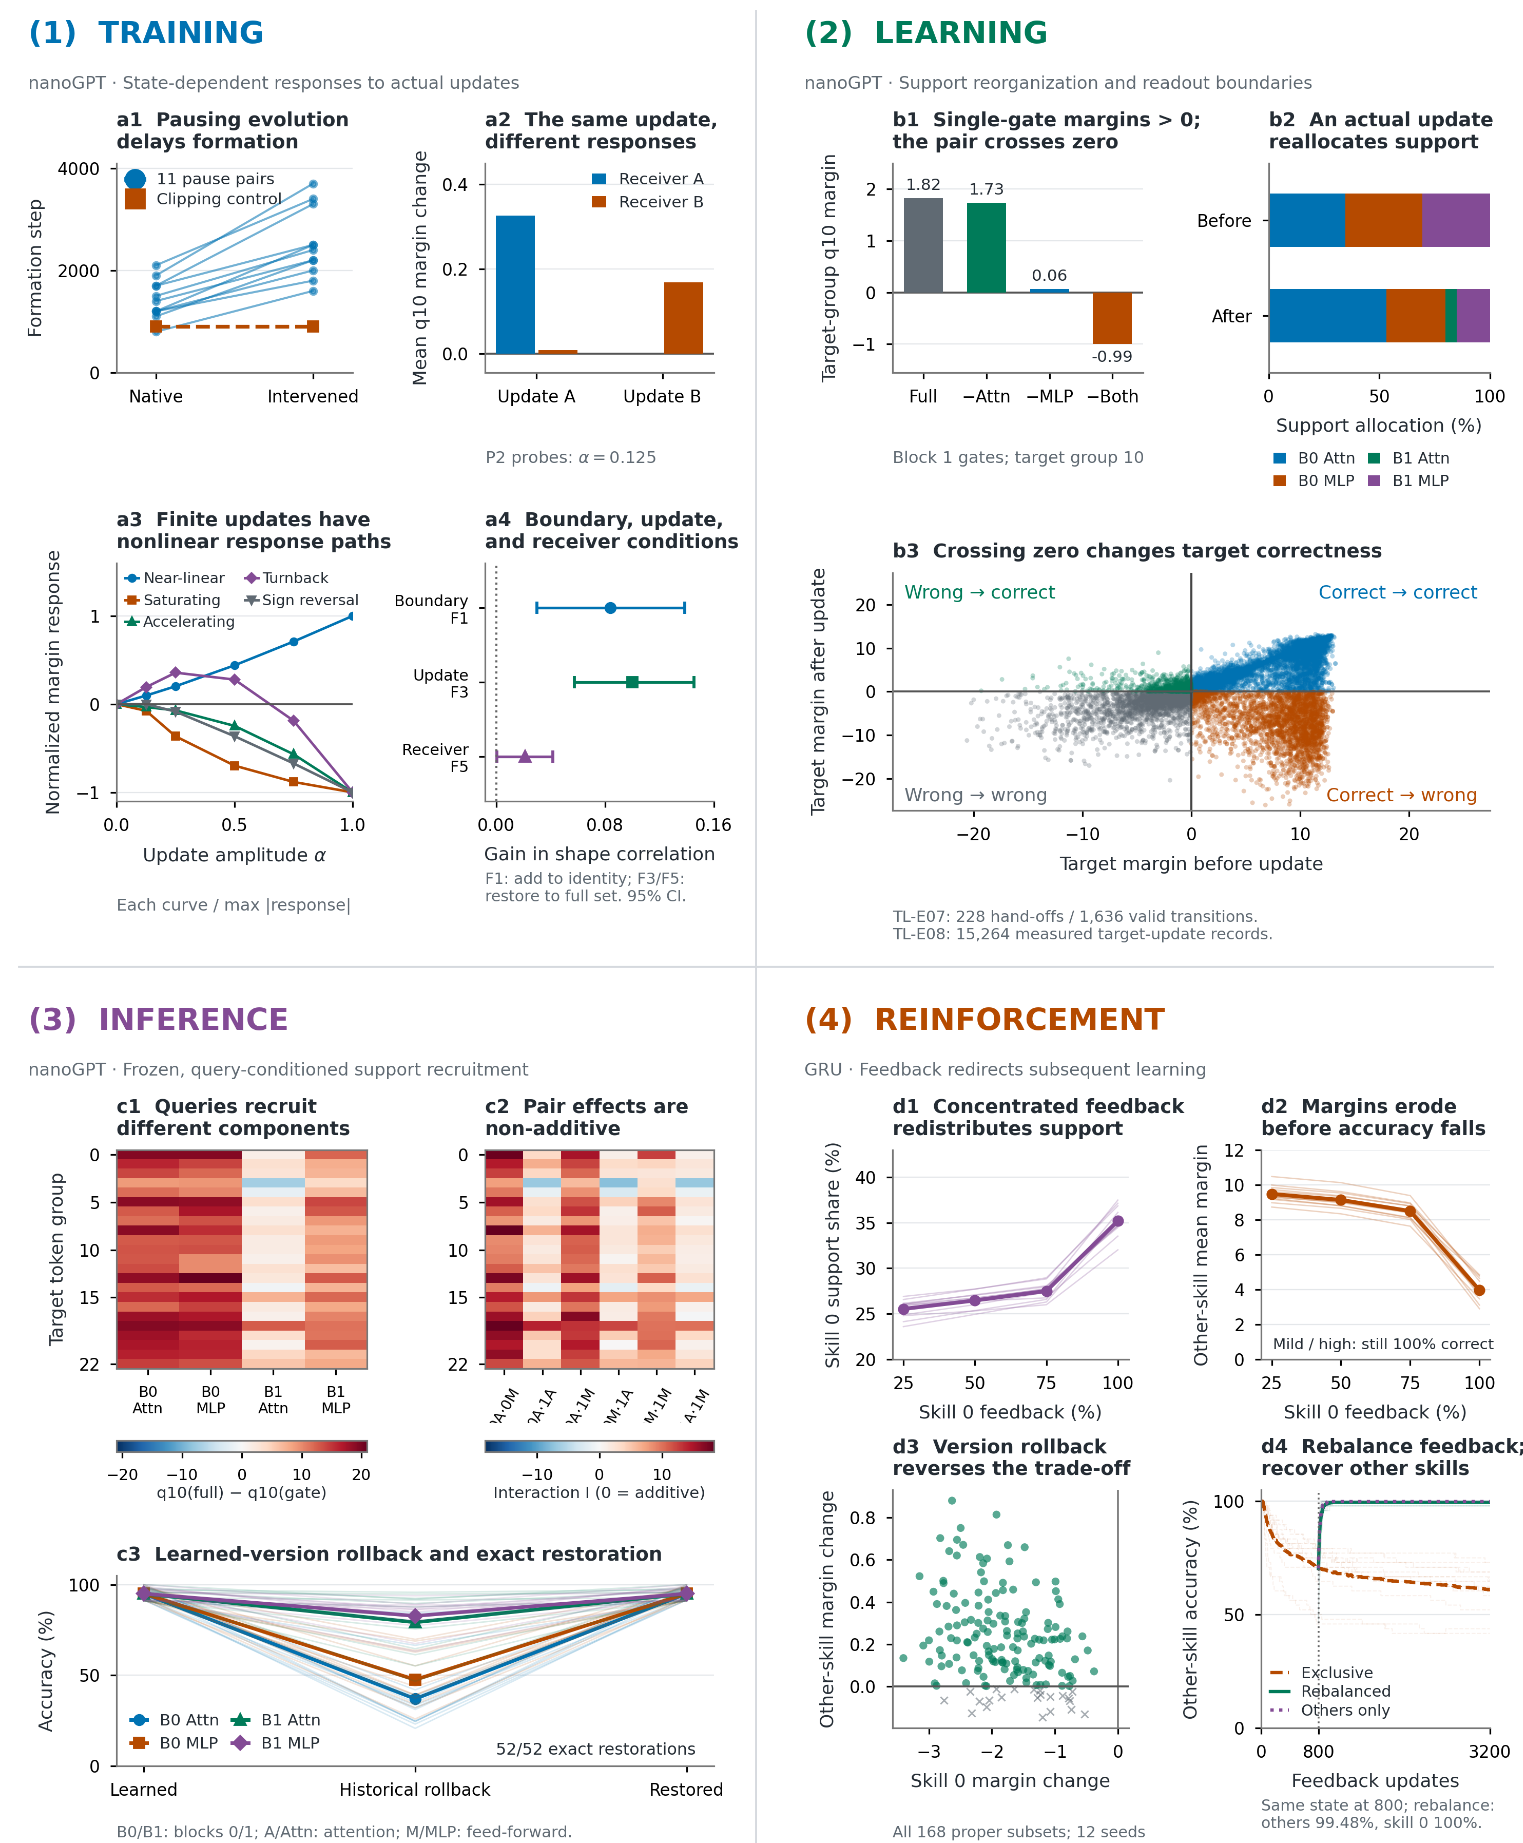
\includegraphics[width=1.00\textwidth,height=.63\textheight,keepaspectratio]{../figures/figure2_experimental_14panel.png}
 \caption{nanoGPT 中训练、学习和冻结推理的代表性实验证据，以及共享 GRU 中反馈驱动的能力变化与恢复。
 (a1) 暂停演化延迟能力形成；
 (a2) 相同真实更新在不同接收状态下引起不同响应；
 (a3) 有限幅度响应的不同类型；
 (a4) 边界、更新和接收状态三类条件因素。
 (b1) 联合移除组件导致目标跨越边界；
 (b2) 一次真实更新引起功能支撑重新分配；
 (b3) 更新前后的目标间隔。
 (c1) 查询条件依赖的组件效应；
 (c2) 非加性成对交互；
 (c3) 已学习组件版本回退与精确恢复。
 (d1) 反馈剂量下的支撑重分配；
 (d2) 准确率下降前的间隔侵蚀；
 (d3) 回退引起的能力权衡；
 (d4) 反馈重新均衡及能力恢复。}
 \label{fig:tlir-evidence}
\end{figure}

\begin{figure}[!htbp]
 \centering
 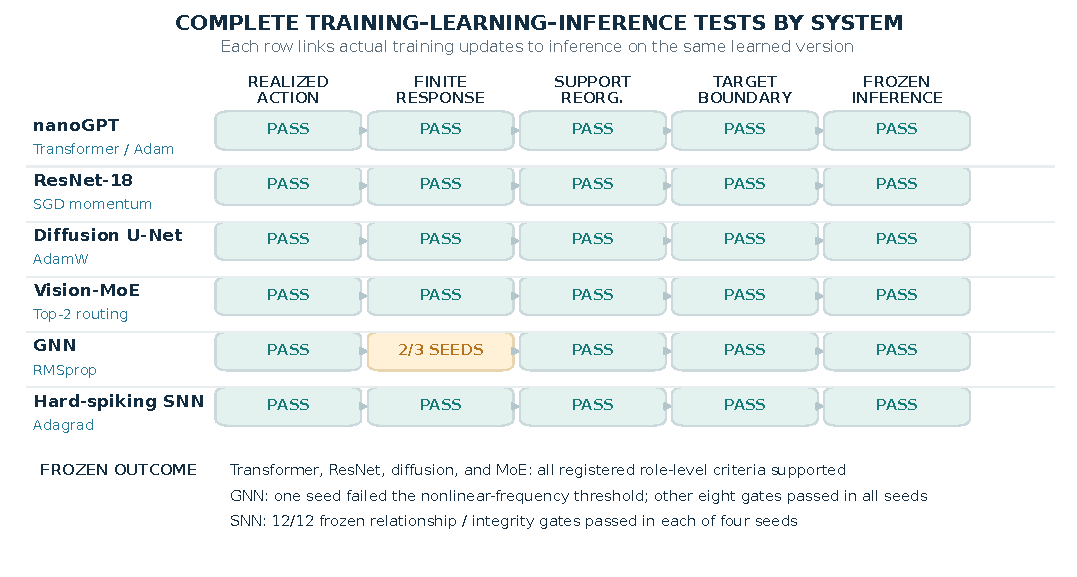
\includegraphics[width=.98\textwidth]{../figures/figure2_six_system_evidence.pdf}
 \caption{六种神经系统各自内部的训练—学习—推理实验关系链。GNN 中有一个随机种子满足九项注册判据中的八项，其非线性响应发生频率低于规定阈值；SNN 在四个随机种子中全部通过十二项注册判据。}
 \label{fig:systems}
\end{figure}

\begin{table}[!htbp]
\caption{七种神经系统：六条 TLI 实验链及一项 GRU 反馈研究。}
\label{tab:systems}
\centering\small\setlength{\tabcolsep}{3pt}\renewcommand{\arraystretch}{1.20}
\begin{tabular}{@{}>{\raggedright\arraybackslash}p{.43\columnwidth}>{\raggedright\arraybackslash}p{.53\columnwidth}@{}}
\toprule
系统（优化器） & 任务／注册组件\\
\midrule
nanoGPT（Adam） & 循环式下一词元预测；4 个注意力／MLP 分支\\
ResNet-18（SGD momentum） & CIFAR-100 分类；4 个残差阶段\\
Diffusion U-Net（AdamW） & CIFAR-10 去噪；4 条 U-Net 路径\\
Vision-MoE（AdamW） & CIFAR-100 分类；4 个路由专家\\
GNN（RMSprop） & 图可达性判断；4 个消息传递模块\\
Spiking SNN（Adagrad） & $8\times8$ 数字图像；4 个脉冲模块\\
GRU（RL-E05/E06；AdamW） & 四技能反馈；4 个共享隐藏状态组\\
\bottomrule
\end{tabular}
\end{table}

\begin{table}[!htbp]
\caption{更新后目标边界分类结果。宏平均召回率为四种实际观察到的能力转变类别的平均召回率；仅有较高准确率并不足以说明预测性能。各系统的预测方法细节与评价集合有所不同。}
\label{tab:prediction}
\centering\small\setlength{\tabcolsep}{4.2pt}\renewcommand{\arraystretch}{1.15}
\begin{tabular}{@{}lrr@{}}
\toprule
系统 & 准确率（\%） & 四类别宏平均召回率（\%）\\
\midrule
nanoGPT & 91.43 & 91.49\\
ResNet-18 & 99.28 & 97.99\\
Diffusion U-Net & 99.60 & 97.98\\
Vision-MoE & 99.63 & 96.95\\
GNN$^{a}$ & 98.54 & 98.62\\
Hard-spiking SNN$^{a}$ & 95.31 & 70.74\\
\bottomrule
\multicolumn{3}{@{}p{.94\columnwidth}@{}}{\footnotesize $^{a}$ GNN 与 SNN 的独立预测检验使用已注册的训练历史。}\\
\end{tabular}
\end{table}

\begin{table}[!htbp]
\caption{RL-E06 每次更新中分配给四项能力的反馈回合数。}
\label{tab:dose}
\centering\small\setlength{\tabcolsep}{4.1pt}\renewcommand{\arraystretch}{1.13}
\begin{tabular}{@{}lrrrr@{}}\toprule
反馈方式 & $q_0$ & $q_1$ & $q_2$ & $q_3$\\\midrule
均衡（Balanced） & 15 & 15 & 15 & 15\\
轻度集中（Mild） & 30 & 10 & 10 & 10\\
高度集中（High） & 45 & 5 & 5 & 5\\
独占（Exclusive） & 60 & 0 & 0 & 0\\\bottomrule
\end{tabular}
\end{table}

\newpage
\input{../references.bbl}

\section*{投稿声明}

\noindent\textbf{资金支持。}
本研究未获得任何资金资助。

\noindent\textbf{作者贡献。}
Mian Wang 提出研究构想；建立原子生成事实模型、生成事实图（GFG）、基于 GFG 的递归科学研究过程，以及训练—学习—推理—强化统一理论；确定科学问题、研究边界与决策标准；提出主要理论假设和概念转换；主导研究计划；分析并解释经过验证的结果；提出前瞻性预测和理论推导；制作图表；撰写并修改论文。

\noindent\textbf{利益冲突。}
作者声明不存在利益冲突。

\noindent\textbf{数据、代码与材料可用性。}
本研究的公开证据仓库按照论文的科学主张组织，旨在支持快速机器辅助审计（\url{https://github.com/wind342/tlir-research-evidence/tree/codex/tlir-paper-evidence-navigation-v1}）。论文—证据映射将主要科学主张、实验、图中子图和报告结果，与冻结协议、源代码、结果记录、来源及校验和清单、独立验证程序建立对应关系。公开证据矩阵还说明了哪些结果能够独立重新计算，以及哪些底层检查点或运行材料没有包含在公开发布的版本中。

\noindent\textbf{生成式人工智能的使用与贡献。}
包括 OpenAI Codex 和 ChatGPT 在内的通用 AI 系统，在基于 GFG 的递归科学研究过程中充当科研代理。在作者的指导下，这些 AI 系统\textbf{发明并实现了四套实验仪器}——CSRG-4C、真实更新因果分叉仪器、有限幅度更新路径仪器和身份对齐目标边界账本——并且设计、实现、启动、监控和执行了论文报告的实验。AI 系统开展了分析、因果干预、匹配重放、反例搜索和独立验证，并参与论文起草、编辑和 LaTeX 排版。所有报告的数值结果均由记录在案的原生程序与执行环境产生，而非 AI 模型直接生成的文本。作者确定科学问题、研究边界和决策标准，审查经过验证的证据，并对科学主张与结果承担责任。
